% torchtest2 tutorial for students and PhD students.
% Build: tectonic torchtest2_tutorial.tex   (or: latexmk -pdf torchtest2_tutorial.tex)
\documentclass[aspectratio=169,11pt]{beamer}
\usetheme{metropolis}
\usepackage{booktabs}
\usepackage{listings}
\usepackage{xcolor}
\usepackage{graphicx}

\definecolor{codebg}{HTML}{F4F4F2}
\definecolor{kw}{HTML}{256ABF}
\definecolor{cm}{HTML}{6B6A66}
\definecolor{st}{HTML}{8A4B00}
\definecolor{pass}{HTML}{1B7F4C}
\definecolor{warn}{HTML}{B86E00}
\definecolor{fail}{HTML}{C0392B}
\lstset{
  language=Python, basicstyle=\ttfamily\fontsize{7}{8.2}\selectfont, backgroundcolor=\color{codebg},
  keywordstyle=\color{kw}\bfseries, commentstyle=\color{cm}\itshape, stringstyle=\color{st},
  showstringspaces=false, frame=none, xleftmargin=3pt, xrightmargin=3pt,
  aboveskip=3pt, belowskip=3pt, columns=fullflexible, keepspaces=true,
}
\lstdefinestyle{report}{language={}, basicstyle=\ttfamily\fontsize{5.4}{6.3}\selectfont, keywordstyle={},
  commentstyle={}, stringstyle={}}
\lstdefinestyle{shell}{language=bash, morekeywords={pip,pytest}}
\newcommand{\PASS}{\textcolor{pass}{\texttt{PASS}}}
\newcommand{\WARN}{\textcolor{warn}{\texttt{WARN}}}
\newcommand{\FAIL}{\textcolor{fail}{\texttt{FAIL}}}
\newcommand{\SKIP}{\textcolor{gray}{\texttt{SKIP}}}
\newcommand{\chk}[1]{\texttt{#1}}
\newcommand{\tool}{\textsf{torchtest2}}
\setbeamersize{text margin left=0.55cm, text margin right=0.55cm}

\title{\tool: testing PyTorch models\\before you train them}
\subtitle{A practical tutorial for students and PhD students}
\author{Grzegorz Gwardys}
\institute{Warsaw University of Technology \;\textbullet\; Promity}
\date{}

\begin{document}

\maketitle

% ------------------------------------------------------------------------------------------------
\section{Why test a model before training?}

\begin{frame}{Silent bugs}
  Many deep-learning bugs do \alert{not crash}. The code runs, the loss goes down a bit, and the
  bug shows up---if ever---after days of GPU time.
  \medskip
  \begin{itemize}
    \item a layer that is defined but \alert{never used} in \texttt{forward}
    \item an optimizer created \alert{before the head was replaced}
    \item \texttt{.detach()} / \texttt{.data} / \texttt{.item()} that \alert{cuts the graph}
    \item an RNN or attention layer that treats the \alert{batch as time}
          (\texttt{batch\_first} mix-up)
    \item an attention \alert{mask that is ignored}
    \item dropout that \alert{stays on at inference}
  \end{itemize}
  None of these raises an exception. Most of them do not even stop the loss from decreasing.
\end{frame}

\begin{frame}[fragile]{Folklore, packaged into one call}
  Experienced practitioners run sanity checks by hand:
  \begin{itemize}
    \item ``check the loss at initialisation'', ``overfit a single batch'' (Karpathy)
    \item ``check that all variables change'' (mltest, torchtest)
    \item ``check that samples do not influence each other'' (Krokotsch)
  \end{itemize}
  \medskip
  \tool{} runs \alert{18 such checks} on \alert{one batch}, in \alert{seconds}, with
  \alert{one call}, and explains every finding:
  \begin{lstlisting}
report = torchtest2.check_model(model, inputs, targets,
                                loss_fn=F.cross_entropy, optimizer=optimizer)
print(report)   # PASS / WARN / FAIL / SKIP for each check, with a message
  \end{lstlisting}
  It is meant to live in your \alert{unit tests}, next to the model code---before a training
  pipeline even exists.
\end{frame}

% ------------------------------------------------------------------------------------------------
\section{First steps}

\begin{frame}[fragile]{Installation}
  \begin{lstlisting}[style=shell]
pip install torchtest2
  \end{lstlisting}
  \begin{itemize}
    \item Python $\geq$ 3.10, PyTorch $\geq$ 2.1, \alert{no other dependencies}
    \item works on CPU and GPU; inputs and targets are moved to the model's device
  \end{itemize}
  \medskip
  The minimum call needs only a model and a batch:
  \begin{lstlisting}
torchtest2.check_model(model, inputs)
  \end{lstlisting}
  Without a loss function the loss-based checks are skipped and the gradient checks use a random
  projection of the outputs instead. Give the loss and the optimizer you really train with to get
  all checks.
\end{frame}

\begin{frame}[fragile]{A model with a bug}
  \begin{lstlisting}
import torch, torch.nn as nn, torch.nn.functional as F
import torchtest2

class Classifier(nn.Module):
    def __init__(self):
        super().__init__()
        self.encoder = nn.Sequential(nn.Linear(32, 64), nn.ReLU())
        self.norm = nn.LayerNorm(64)          # defined...
        self.head = nn.Linear(64, 10)

    def forward(self, x):
        return self.head(self.encoder(x))     # ...but never used
torch.manual_seed(0)
model = Classifier()
optimizer = torch.optim.Adam(model.parameters(), lr=1e-3)
x, y = torch.randn(16, 32), torch.randint(0, 10, (16,))

report = torchtest2.check_model(model, x, y, loss_fn=F.cross_entropy, optimizer=optimizer)
print(report)
  \end{lstlisting}
\end{frame}

\begin{frame}[fragile]{The report}
  \begin{lstlisting}[style=report]
torchtest2 report for Classifier  (parameters: 2,890, trainable: 2,890, device: cpu, batch size: 16, objective: loss_fn)
  PASS  forward             output: Tensor[16, 10] float32
  SKIP  output_shape        no output_shape given
  PASS  output_finite       no NaN/inf in the outputs
  SKIP  output_range        no output_range given
  PASS  output_varies       outputs differ between samples
  PASS  eval_determinism    eval-mode forward passes are reproducible
  PASS  loss                loss = 2.323 (loss_fn)
  PASS  initial_loss        initial loss 2.323 is close to ln(10) = 2.303
  PASS  optimizer_coverage  the optimizer covers every trainable parameter
  FAIL  gradient_flow       2/6 trainable parameter(s) get no gradient from the loss_fn (unused in
                            forward, or the graph is cut by .detach()/.item()/no_grad): norm.weight, norm.bias
  PASS  gradient_magnitude  total gradient norm 0.949
  FAIL  params_change       2/6 trainable parameter(s) did not change after an optimizer step: norm.weight, norm.bias
  SKIP  frozen_params       no frozen parameters (requires_grad=False or frozen=[...])
  PASS  input_dependency    all 1 input tensor(s) influence the output
  PASS  batch_independence  outputs of a sample do not depend on other samples in the batch (eval mode)
  PASS  overfit_batch       loss 2.323 -> 0.2244 in 85 step(s)
  SKIP  gpu                 require_gpu=False
  11 passed, 0 warnings, 2 failed, 4 skipped
  \end{lstlisting}
  \small Every finding \alert{names the offending parameters} and suggests likely causes.
\end{frame}

\begin{frame}{Four statuses}
  \centering
  \begin{tabular}{ll}
    \toprule
    Status & Meaning \\
    \midrule
    \PASS & nothing suspicious \\
    \WARN & suspicious, but can be legitimate: \alert{read the message} \\
    \FAIL & almost certainly a bug \\
    \SKIP & not applicable (e.g.\ no loss given) or disabled \\
    \bottomrule
  \end{tabular}
  \bigskip
  \begin{itemize}
    \item \texttt{report.ok} is \texttt{True} when nothing \FAIL{}ed (warnings are allowed)
    \item \texttt{strict=True} turns warnings into failures
    \item why warnings? Some findings are legitimate by design: a zero-initialised head gives
          zero gradients at init, a contrastive model compares samples on purpose
  \end{itemize}
\end{frame}

% ------------------------------------------------------------------------------------------------
\section{The most important checks}

\begin{frame}{All 18 checks at a glance}
  \scriptsize
  \begin{tabular}{p{0.12\linewidth}p{0.43\linewidth}p{0.36\linewidth}}
    \toprule
    Group & Checks & Catches \\
    \midrule
    outputs & \chk{forward}, \chk{output\_shape}, \chk{output\_finite}, \chk{output\_range} &
      crashes, wrong head size, NaN, missing sigmoid \\
     & \chk{output\_varies}, \chk{eval\_determinism} & collapsed outputs, randomness at inference \\
    loss & \chk{loss}, \chk{initial\_loss} & unreduced loss, over-confident init \\
    optimisation & \chk{optimizer\_coverage}, \chk{params\_change}, \chk{frozen\_params} &
      stale optimizer, \texttt{lr=0}, a ``frozen'' layer that trains \\
    gradients & \chk{gradient\_flow}, \chk{gradient\_magnitude} & unused layers, cut graph, NaN \\
    data flow & \chk{input\_dependency}, \chk{batch\_independence} &
      ignored inputs/masks, samples leaking \\
    training & \chk{overfit\_batch} & anything that prevents learning \\
    opt-in & \chk{gradcheck}, \chk{gpu} & wrong custom \texttt{backward}, training on CPU \\
    \bottomrule
  \end{tabular}
  \medskip

  \small The next slides show the checks that catch the most common silent bugs.
\end{frame}

\begin{frame}{Which checks run the model, and how}
  \centering
  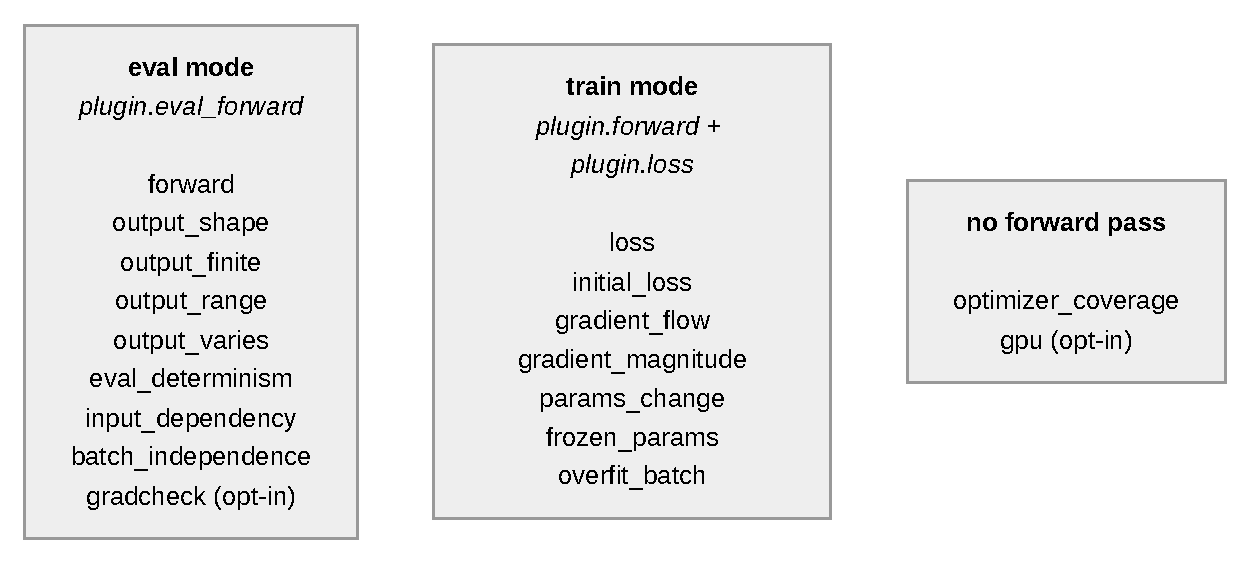
\includegraphics[width=0.78\textwidth]{../diagrams/checks_by_mode.pdf}
  \medskip

  \small Inference checks run in \alert{eval mode} (so BatchNorm's batch statistics and dropout are
  off), training checks in \alert{train mode}. The plugin section shows which plugin method each
  mode uses.
\end{frame}

\begin{frame}[fragile]{\chk{optimizer\_coverage}: the fine-tuning classic}
  \begin{lstlisting}
model = nn.Sequential(nn.Linear(32, 64), nn.ReLU(), nn.Linear(64, 1000))  # "pretrained"
optimizer = torch.optim.AdamW(model.parameters(), lr=1e-3)
model[2] = nn.Linear(64, 10)            # new head for 10 classes - AFTER the optimizer

report = check_model(model, x, y, loss_fn=F.cross_entropy, optimizer=optimizer)
  \end{lstlisting}
  \begin{lstlisting}[style=report]
FAIL  optimizer_coverage  2 trainable parameter(s) are not in the optimizer: 2.weight, 2.bias. The optimizer
                          holds 2 tensor(s) that are not (or no longer) parameters of this model - were layers
                          replaced after creating it, or was it created for another model instance?
FAIL  params_change       2/4 trainable parameter(s) did not change after an optimizer step: 2.weight, 2.bias
  \end{lstlisting}
  \begin{itemize}
    \item the new head \alert{is never trained}; the loss still goes down a little
    \item \chk{optimizer\_coverage} compares parameter \emph{identities} with the optimizer's
          parameter groups---it needs \alert{your} optimizer
  \end{itemize}
\end{frame}

\begin{frame}[fragile]{\chk{gradient\_flow} and \chk{params\_change}: a cut graph}
  \begin{lstlisting}
class Net(nn.Module):
    def __init__(self):
        super().__init__()
        self.backbone = nn.Linear(32, 64)
        self.head = nn.Linear(64, 10)

    def forward(self, x):
        features = self.backbone(x).data     # legacy .data silently detaches
        return self.head(F.relu(features))
  \end{lstlisting}
  \begin{lstlisting}[style=report]
FAIL  gradient_flow  2/4 trainable parameter(s) get no gradient from the loss_fn (unused in forward, or the
                     graph is cut by .detach()/.item()/no_grad): backbone.weight, backbone.bias
  \end{lstlisting}
  \begin{itemize}
    \item \texttt{None} gradient $\Rightarrow$ \FAIL{} (unused, or the graph is cut)
    \item all-zero gradient $\Rightarrow$ \WARN{} (zero-initialised layers are legitimate)
    \item \chk{params\_change}: one step with \alert{your} optimizer must change every
          trainable parameter (catches \texttt{lr=0}, too)
  \end{itemize}
\end{frame}

\begin{frame}[fragile]{\chk{batch\_independence}: samples must not talk to each other}
  \begin{lstlisting}
class Encoder(nn.Module):
    def __init__(self, dim=16, heads=4):
        super().__init__()
        self.attn = nn.MultiheadAttention(dim, heads)   # batch_first=False by default!
        self.out = nn.Linear(dim, dim)

    def forward(self, x):                                 # x: (batch, tokens, dim)
        h, _ = self.attn(x, x, x)
        return self.out(h)

report = check_model(Encoder(), torch.randn(4, 6, 16))
  \end{lstlisting}
  \begin{lstlisting}[style=report]
FAIL  batch_independence  changing sample 0 changed the outputs of 3/3 other sample(s), e.g. [1, 2, 3]: the
                          model mixes information across the batch (view/reshape instead of transpose/permute,
                          a batch_first mix-up, softmax or normalisation over the batch dimension?)
  \end{lstlisting}
  \small How: replace sample 0 by sample 1 and check, in eval mode, that the outputs of samples
  $1\ldots N{-}1$ do not change. Works for token ids, masks and any output structure.
\end{frame}

\begin{frame}[fragile]{\chk{input\_dependency}: is every input actually used?}
  \begin{lstlisting}
class TwoTower(nn.Module):
    def __init__(self):
        super().__init__()
        self.user = nn.Linear(16, 8)
        self.item = nn.Linear(16, 8)

    def forward(self, x):                      # x = [user features | item features]
        u, i = x[:, :16], x[:, 16:]
        return (self.user(u) * self.item(u)).sum(-1)    # BUG: item tower gets user features
  \end{lstlisting}
  \begin{lstlisting}[style=report]
FAIL  input_dependency  16/32 features of inputs (per-sample shape (32,)) have no influence on the output,
                        e.g. at [(16,), (17,), (18,)] (wrong slice/split, a variable reused by mistake?)
  \end{lstlisting}
  \begin{itemize}
    \item float inputs: gradient per \alert{feature}; integer and boolean inputs (token ids,
          attention masks) are rolled along the batch and must change the output
    \item catches ignored attention masks in Hugging Face-style \texttt{dict} inputs too
  \end{itemize}
\end{frame}

\begin{frame}{Three more checks worth knowing}
  \begin{description}[\chk{eval\_determinism}]
    \item[\chk{eval\_determinism}] two forward passes in eval mode must agree. \WARN{} for
      \texttt{F.dropout(x)} without \texttt{training=self.training}, or \texttt{torch.rand} in
      \texttt{forward}.
    \item[\chk{initial\_loss}] cross-entropy at initialisation should be close to
      $\ln C$. \WARN{} for an over-confident initialisation (or label leakage).
    \item[\chk{overfit\_batch}] trains on the one batch until the loss falls to 10\,\% of its
      initial value; checks that gradients stay finite \alert{at every step}. Catches anything
      that prevents learning, and NaN gradients that appear only after a few updates.
  \end{description}
  \bigskip
  \small \chk{overfit\_batch} is the slowest check (up to \texttt{overfit\_steps=200}); lower it,
  or \texttt{skip=["overfit\_batch"]} while iterating.
\end{frame}

\begin{frame}{What happens inside \texttt{check\_model}}
  \centering
  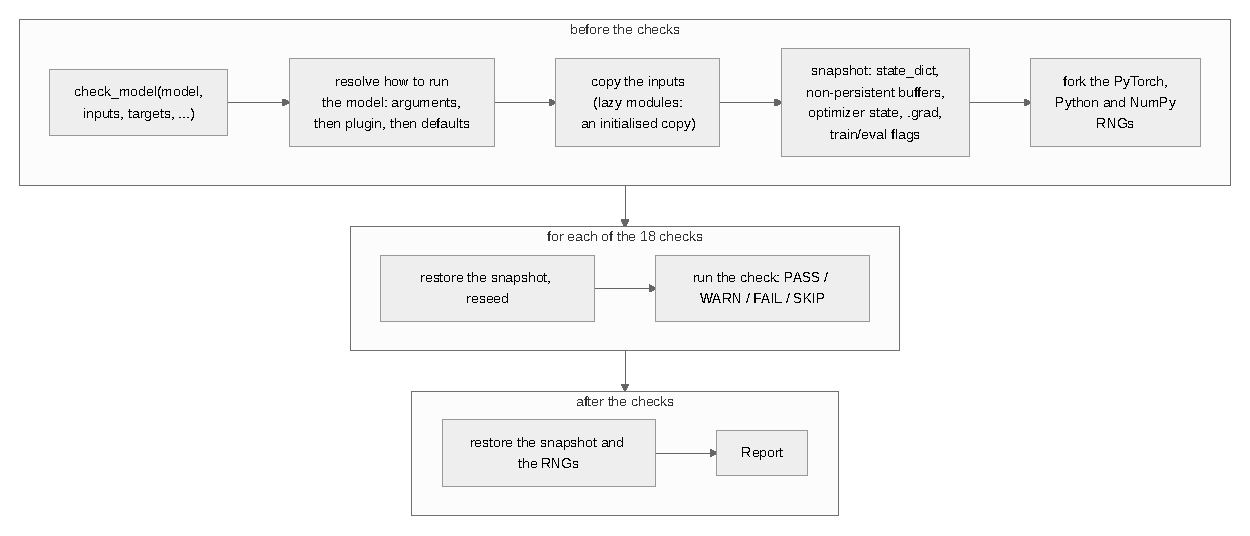
\includegraphics[height=0.80\textheight]{../diagrams/check_model_lifecycle.pdf}
\end{frame}

\begin{frame}{It does not touch your objects}
  \tool{} restores the PyTorch state it touches after every check:
  \begin{itemize}
    \item parameters, buffers (also non-persistent ones), optimizer state, \texttt{.grad} tensors,
          train/eval flags, uninitialised lazy modules
    \item the PyTorch, Python and NumPy random generators
    \item your input tensors are copied, so in-place operations in \texttt{forward} cannot change
          them
  \end{itemize}
  \medskip
  So you can call it anywhere in a test suite---even on the model you are about to train.
  \medskip

  \small Not restored: plain Python attributes that your own \texttt{forward} changes (e.g.\ a call
  counter).
\end{frame}

% ------------------------------------------------------------------------------------------------
\section{Running checks in a test suite}

\begin{frame}[fragile]{pytest: one line per architecture}
  \begin{lstlisting}
import pytest, torch, torch.nn.functional as F            # tests/test_models.py
import torchtest2
from my_project.models import build_model            # your code

@pytest.mark.parametrize("arch", ["resnet18", "vit_tiny", "my_new_idea"])
def test_architecture_is_trainable(arch):
    torch.manual_seed(0)
    model = build_model(arch, num_classes=10)
    x, y = torch.randn(8, 3, 64, 64), torch.randint(0, 10, (8,))
    optimizer = torch.optim.AdamW(model.parameters(), lr=3e-4)
    torchtest2.assert_model_ok(model, x, y, loss_fn=F.cross_entropy, optimizer=optimizer,
                               output_shape=(None, 10), overfit_steps=100)
  \end{lstlisting}
  \begin{lstlisting}[style=shell]
pytest tests/test_models.py
  \end{lstlisting}
  \small \texttt{assert\_model\_ok} raises \texttt{ModelCheckError} (an \texttt{AssertionError})
  listing the failed checks and the whole report, so pytest shows it as a test failure.
\end{frame}

\begin{frame}[fragile]{Tuning the checks to your model}
  \begin{lstlisting}
# warnings are failures, too
torchtest2.assert_model_ok(model, x, y, loss_fn=F.cross_entropy, strict=True)

# a contrastive model compares the samples of a batch on purpose
torchtest2.assert_model_ok(model, x, skip=["batch_independence"])

# a frozen backbone must not change; outputs must be probabilities
torchtest2.assert_model_ok(model, x, y, loss_fn=F.nll_loss,
                           frozen=["backbone"], output_range=(0, 1))

# sequence-first RNN: inputs (time, batch, features), outputs (batch, classes)
torchtest2.assert_model_ok(model, x, batch_dim=1, output_batch_dim=0)
# assert on single checks
report = torchtest2.check_model(model, x, y, loss_fn=F.cross_entropy)
assert report["gradient_flow"].status is torchtest2.Status.PASS
  \end{lstlisting}
  \small Tip: use a \alert{small configuration} of your architecture (few layers, narrow width)
  and a batch of 4--16 distinct samples. Most bugs do not depend on size.
\end{frame}

\begin{frame}[fragile]{The class-based API: \texttt{ModelTester} and \texttt{TestSuite}}
  \begin{lstlisting}
from torchtest2 import ModelTester, TestSuite

batch = [torch.randn(32, 1, 28, 28), torch.randint(0, 10, (32,))]
model = nn.Sequential(nn.Flatten(), nn.Linear(784, 64), nn.ReLU(), nn.Linear(64, 10))
optimizer = torch.optim.Adam(model.parameters(), lr=1e-2)

tester = ModelTester(model, F.cross_entropy, optimizer, batch)
tester.test_parameters_change()      # one test; raises ParametersChangeException
tester.test_batch_independence()     # raises BatchIndependencyException
report = tester.check()              # the full check_model report
suite = TestSuite(model, F.cross_entropy, optimizer, batch,
                  test_suite_config={"test_parameters_change": True,
                                     "test_input_dependency": True,
                                     "test_overfit": True})
results = suite.test_suite()         # runs ALL enabled tests, prints a summary -> {test: passed}
  \end{lstlisting}
  \small \texttt{ModelTester.test\_suite()} stops at the first failure; \texttt{TestSuite}
  collects all results---useful in notebooks and reports.
\end{frame}

% ------------------------------------------------------------------------------------------------
\section{Plugins}

\begin{frame}{Why plugins?}
  Not every model is trained through \texttt{loss\_fn(model(inputs), targets)}:
  \begin{itemize}
    \item \alert{detection models} take the targets in training mode and return a dict of losses
    \item \alert{Hugging Face} models compute their own loss from \texttt{labels=}
    \item \alert{Lightning} modules define \texttt{training\_step} and
          \texttt{configure\_optimizers}
    \item your lab's multi-task models do something else again
  \end{itemize}
  \medskip
  A plugin answers \alert{``how is this family of models run?''}---training forward, eval
  forward, loss, optimizer, batch dimensions.
  \medskip

  The checks themselves stay \alert{the same for every model}: a plugin never decides what is
  checked, only how the model is executed. That keeps reports comparable across model families.
\end{frame}

\begin{frame}{Built-in plugins}
  \scriptsize
  \begin{tabular}{p{0.26\linewidth}p{0.23\linewidth}p{0.41\linewidth}}
    \toprule
    Name & For & What it does \\
    \midrule
    \texttt{"torchvision\_detection"} & Faster/Mask R-CNN, RetinaNet, FCOS, SSD, \ldots &
      train: \texttt{model(images, targets)} and the sum of the loss dict; eval:
      \texttt{model(images)}; a list of images has no batch dimension \\
    \texttt{"huggingface"} & \texttt{transformers} models &
      train: \texttt{model(**inputs, labels=targets)} and \texttt{outputs.loss} \\
    \texttt{"lightning"} & \texttt{LightningModule}s &
      train: \texttt{training\_step((inputs, targets), 0)} and the loss it returns; optimizer
      from \texttt{configure\_optimizers()} \\
    \bottomrule
  \end{tabular}
  \bigskip

  \normalsize
  \begin{itemize}
    \item select by name: \texttt{check\_model(model, x, y, plugin="lightning")}
    \item none of them imports its framework: \tool{} still depends only on PyTorch
    \item explicit arguments (\texttt{optimizer=}, \texttt{loss\_fn=}, \ldots) win over the plugin
  \end{itemize}
\end{frame}

\begin{frame}[fragile]{Using a ready-made plugin: PyTorch Lightning}
  \begin{lstlisting}
import lightning as L

class LitClassifier(L.LightningModule):
    def __init__(self):
        super().__init__()
        self.net = nn.Sequential(nn.Linear(32, 64), nn.ReLU(), nn.Linear(64, 10))
        self.aux_head = nn.Linear(64, 10)                 # added later...

    def forward(self, x):
        return self.net(x)
    def training_step(self, batch, batch_idx):
        x, y = batch
        loss = F.cross_entropy(self(x), y)
        self.log("train_loss", loss)                      # harmless outside a Trainer
        return loss
    def configure_optimizers(self):
        return torch.optim.Adam(self.net.parameters(), lr=1e-3)   # ...but not optimised

report = check_model(LitClassifier(), x, y, plugin="lightning")   # report on the next slide
  \end{lstlisting}
\end{frame}

\begin{frame}[fragile]{The Lightning plugin: report, details and limits}
  \begin{lstlisting}[style=report]
FAIL  optimizer_coverage  2 trainable parameter(s) are not in the optimizer: aux_head.weight, aux_head.bias.
                          Was the optimizer created before these layers were added/replaced?
  \end{lstlisting}
  \begin{itemize}
    \item it calls \alert{your} \texttt{training\_step} and uses the first optimizer of
          \texttt{configure\_optimizers()}, as the trainer would
    \item a different batch structure? Tell the plugin how to build it:
  \end{itemize}
  \begin{lstlisting}
from torchtest2.plugins import LightningPlugin

plugin = LightningPlugin(make_batch=lambda inputs, targets: {"x": inputs, "y": targets})
check_model(module, x, y, plugin=plugin)
  \end{lstlisting}
  \begin{itemize}
    \item it supports \alert{common} \texttt{LightningModule} patterns; it does \alert{not}
          reproduce the Trainer: no strategies or distributed execution, precision plugins,
          manual optimisation, several optimizers, schedulers, gradient accumulation or callbacks
  \end{itemize}
\end{frame}

\begin{frame}[fragile]{A model that does not fit the default}
  \begin{lstlisting}
class MultiTask(nn.Module):
    def __init__(self):
        super().__init__()
        self.body, self.cls, self.aux = nn.Linear(32, 64), nn.Linear(64, 10), nn.Linear(64, 1)
    def forward(self, x, y=None):
        h = F.relu(self.body(x))
        if y is None:                     # inference:  model(x)    -> logits
            return self.cls(h)
        return {"cls": F.cross_entropy(self.cls(h), y),           # training: model(x, y)
                "aux": self.aux(h).pow(2).mean()}                 #   -> a dict of LOSSES
  \end{lstlisting}
  By default, \tool{} trains through \texttt{loss\_fn(model(x), y)}---the inference branch, where
  the \texttt{aux} head never runs:
  \begin{lstlisting}[style=report]
FAIL  gradient_flow   2/6 trainable parameter(s) get no gradient from the loss_fn ...: aux.weight, aux.bias
FAIL  params_change   2/6 trainable parameter(s) did not change after an optimizer step: aux.weight, aux.bias
  \end{lstlisting}
  \small A false alarm: in real training \texttt{aux} \emph{is} trained. \tool{} has to call the
  model the way you train it.
\end{frame}

\begin{frame}[fragile]{How \tool{} uses a plugin}
  \begin{lstlisting}
# every training-mode check (loss, gradients, optimizer steps, overfitting):
train_out = plugin.forward(model, inputs, targets)   # whatever your model returns in training
loss      = plugin.loss(train_out, targets, loss_fn)  # turn THAT into one scalar -> backward()

# every eval-mode check (outputs, input dependency, batch independence):
outputs   = plugin.eval_forward(model, inputs)
  \end{lstlisting}
  \begin{itemize}
    \item \texttt{plugin.forward} is \alert{not} your model's \texttt{forward}: it receives the
          model and decides \alert{how to call it}
    \item the first argument of \texttt{plugin.loss} is \alert{exactly what
          \texttt{plugin.forward} returned}---logits for most models, but for \texttt{MultiTask}
          a dict of losses
    \item \texttt{loss\_fn} is the loss function given by the user, if any; a plugin may ignore it
    \item every method has a default: \texttt{forward} and \texttt{eval\_forward} call
          \texttt{model(inputs)}, \texttt{loss} applies \texttt{loss\_fn} (or uses
          \texttt{outputs.loss})
  \end{itemize}
\end{frame}

\begin{frame}{The plugin calls, step by step}
  \centering
  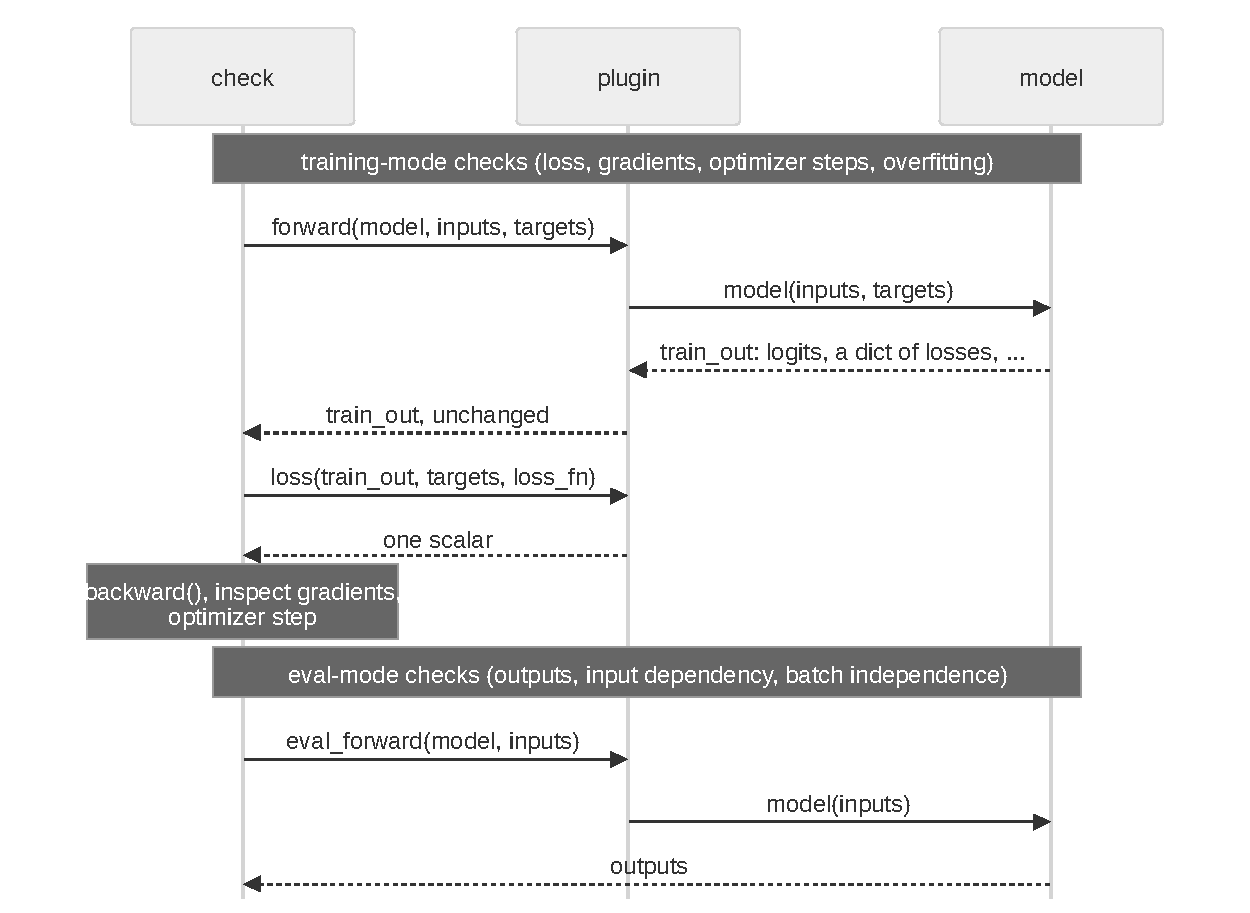
\includegraphics[height=0.80\textheight]{../diagrams/plugin_flow.pdf}
\end{frame}

\begin{frame}[fragile]{Writing your own plugin}
  Subclass \texttt{torchtest2.Plugin} and override only what differs from the default:
  \begin{lstlisting}
from torchtest2 import Plugin

class MultiTaskPlugin(Plugin):
    name = "multitask"
    def forward(self, model, inputs, targets):    # training: call the model WITH the targets
        return model(inputs, targets)              # -> {"cls": ..., "aux": ...}
    def loss(self, losses, targets, loss_fn):      # losses: what forward() returned
        return losses["cls"] + losses["aux"]       # -> one scalar
    # optional: eval_forward (default model(inputs) is right here), configure_optimizer, batch_dim
report = check_model(MultiTask(), x, y, plugin=MultiTaskPlugin())   # all checks pass
  \end{lstlisting}
  \begin{itemize}
    \item \small the same as \texttt{forward\_fn=lambda m, x, y: m(x, y)} plus
          \texttt{loss\_fn=lambda losses, y: ...} in \alert{every} test---written once, for the
          whole model family
  \end{itemize}
\end{frame}

\begin{frame}[fragile]{Sharing a plugin with your lab}
  Register it under the \texttt{torchtest2.plugins} entry-point group of your package:
  \begin{lstlisting}[language={}]
# pyproject.toml of my_lab_tools
[project.entry-points."torchtest2.plugins"]
multitask = "my_lab_tools.testing:MultiTaskPlugin"
  \end{lstlisting}
  After \texttt{pip install my\_lab\_tools}, everyone can write:
  \begin{lstlisting}
check_model(model, x, y, plugin="multitask")
torchtest2.plugin_discovery()     # lists the built-in and installed plugins
  \end{lstlisting}
  \begin{itemize}
    \item names are resolved among the built-in plugins first, then only the requested entry
          point is imported---a broken unrelated plugin cannot break your tests
    \item plugins also work with \texttt{ModelTester} and \texttt{TestSuite} (their
          \texttt{split\_batch} turns a \texttt{batch} into inputs and targets)
  \end{itemize}
\end{frame}

% ------------------------------------------------------------------------------------------------
\section{Wrap-up}

\begin{frame}{What it does not do}
  \begin{itemize}
    \item it tests the \alert{model}, its loss and its optimizer---not your data pipeline,
          training loop, metrics or distributed setup---and most real silent bugs reported
          online live there, outside the model.
    \item \chk{batch\_independence} finds leaks \emph{between} samples, not data scrambled
          \emph{within} a sample
    \item vanishing gradients are not flagged yet (only updates lost to rounding)
    \item a \PASS{} is evidence, not a proof: the checks see one batch, before training
  \end{itemize}
  \medskip
  Think of it as a \alert{linter for model code}: cheap, fast, and it catches the embarrassing
  bugs before they cost you a week of GPU time.
\end{frame}

\begin{frame}{Take-aways and exercises}
  \begin{enumerate}
    \item add \texttt{assert\_model\_ok} to the tests of your current project---one test per
          architecture, with the loss and optimizer you really use
    \item break your model on purpose (\texttt{.detach()} a layer, swap \texttt{batch\_first},
          drop the attention mask) and read what the report says
    \item if you use Lightning or Hugging Face, run the built-in plugin on your module
    \item if your lab has its own training convention, write a plugin and share it as a package
  \end{enumerate}
  \bigskip
  \small Documentation, examples and the bug gallery: the README of the repository.
\end{frame}

\end{document}
